\documentclass{article}
\usepackage[utf8]{inputenc}

\title{Modelling and Estimation of Compliant Carpets}
\author{Daniele Pucci, Silvio Traversaro, Francesco Romano, Francesco Nori}
\date{February 2016}

\usepackage{natbib}
\usepackage{color}

\usepackage{graphicx}
\usepackage{amsmath,amssymb,amsthm}
\newtheorem{assumption}{\bf{Assumption}}
\newtheorem{definition}{\bf{Definition}}
\newtheorem{boldLemma}{\bf{Lemma}}

\begin{document}

\maketitle

\begin{abstract}
    This  document discusses the modelling and estimation of the compliance associated with a soft carpet.
\end{abstract}

\subsection*{Notation}
Throughout the paper we will use the following definitions:
\begin{itemize}
   \item $\mathcal{I}$ denotes an inertial frame, with its $z$ axis pointing against the gravity. %We denote with $g$ the gravitational constant.
    \item $e_i \in \mathbb{R}^m$ is the canonical vector, consisting of all zeros but the $i$-th component which is one.
%    \item Given two orientation frames $A$ and $B$, and vectors of coordinates expressed in these orientation frames, i.e. $\prescript{A}{}p$ and $\prescript{B}{}p$, respectively, the rotation matrix 
    %$\prescript{A}{}R_B$ is such that $\prescript{A}{}p = \prescript{A}{}R_B  \prescript{B}{}p$. 
%    \item $\prescript{A}{}f$ denotes the fact that the vector $f$ is written w.r.t. the frame $A$.
    % \item Given a vector $x \in \mathbb{R}^m$ we denote with $x_i$ its $i$-th element. \marginpar{This notation is used once in this sense in the paper, and multiple times numerical pedices are used with other meanings. I strongly suggest to remove this definition.}
    \item $1_n \in \mathbb{R}^{n \times n}$ is the identity matrix of size $n$; $0_{m \times n} \in \mathbb{R}^{m \times n}$ is the zero matrix of size $m \times n$ and $0_{n } = 0_{n \times 1}$.
    \item We denote with $S(x) \in \mathbb{R}^{3 \times 3}$ the skew-symmetric matrix such that $S(x)y = x \times y$, where $\times$ denotes the cross product operator in $\mathbb{R}^3$. 
    \item Given two vectors $x,y\in \mathbb{R}^n$, their inner product is denoted by $x^\top y$. 
    \item Given a vector of coordinates $v \in \mathbb{R}^n$, we denote with $v_i$ the $i-$th component of this vector, i.e. $v_i = e^\top_i v$.
%    If $x=(\bar{x}^\top,0)^\top$ and $y=(\bar{y}^\top,0)^\top$, with $\bar{x},\bar{y} \in \mathbb{R}^2$ one has $S(x)y = -\bar{x}^\top S \bar{y} e_3$, with 
%    $S = \begin{bmatrix}
%        0 & -1 \\ 1 & 0
%    \end{bmatrix}$.
    % \item $\prescript{A}{}X_B$ is the coordinate transformation from frame $B$ to frame $A$ when applied to motion vectors (e.g. velocities). If we consider a 2D space, $\prescript{A}{}X_B \in \mathbb{R}^{3 \times 3}$.
    % \item $\prescript{A}{}X_B^*$ is the coordinate transformation from frame $B$ to frame $A$ when applied to force vectors (e.g. wrenches). Note that $\prescript{A}{}X_B^* = \prescript{A}{}X_B^{-\top}$. If we consider a 2D space, $\prescript{A}{}X_B^* \in \mathbb{R}^{3 \times 3}$.
\end{itemize}

\section{Modelling}
To introduce the reader to the model of a compliant carpet, we first consider the planar case, and then address the three-dimensional case.

\subsection{A case study: the planar case}

Figure~\ref{fig:compliantCarpet} shows a uniform force distribution acting on a compliant carpet of height~$h$. The resultant force due to the distribution is denoted by $F$. The force distribution induces a compression of the compliant carpet and, assuming uniform carpet characteristics, the  compression is equally distributed. So,  the carpet is horizontal even after the compression due to the force distribution. Now, assume that the mapping $F: z_M \rightarrow F_E$ is known -- or properly estimated --  in the case shown in Figure~\ref{fig:compliantCarpet}. The following details how to evaluate the resultant force and torque acting from the carpet to the contact surface  when it is not uniformly compressed. To this purpose, we make the following assumptions.

 \begin{figure}[t]
     \centering{
     % \includsvg{imgs/model}
         \def\svgwidth{0.85\columnwidth}         
         \input{figures/softFloor.eps_tex}
     \caption{A compliant carpet subject to a uniform force distribution}
     \label{fig:compliantCarpet}
   }
\end{figure}



\begin{assumption}
\label{hp:uniformity} 
Throughout the paper, we assume the following.
\begin{enumerate}
    \item The carpet characteristics are isotropic.
    \item The soft carpet can be approximated as a continuum of springs. In addition, each infinitesimal spring can  exert only a vertical force.
    \item An off-line estimation procedure provides us with the mapping $F = F_E(z_M)$ when a uniform force distribution $f(\cdot)$ is applied to the carpet.
\end{enumerate}
\end{assumption}

Let $l$ denote the length of the compliant carpet subject to the uniform force distribution. As a consequence of assumptions~\ref{hp:uniformity}.1 and~\ref{hp:uniformity}.3, one has:

\begin{equation}
\label{forceFromIntegral}
F_E(z_M) = \int_{a}^{b} f(z_M) dx = f(z_M) l.
\end{equation}
So, we can evaluate the force distribution $f(z)$ from the estimated force $F_E(z_M)$, 

\begin{equation}
f(z) = \frac{F_E(z)}{l}.
\end{equation}

Then, 
Eq.~\eqref{forceFromIntegral} can be used to evaluate  the total force applied from the carpet to a generic contact surface, i.e.

\begin{equation}
\label{forceFromIntegral1}
F = \int_{a}^{b} f(z(x)) dx,
\end{equation}
with $z(x)$  a proper function describing the shape of the  contact surface on a domain $x~\in~[a,b]$.
%, so that $l_n = b-a$. 
Also, in view of the assumption~\ref{hp:uniformity}.2, the torque about a point located at $x = \bar{x}$ of the carpet can  be easily computed as:
\begin{equation}
\label{momentFromIntegral}
M = \int_{a}^{b} f(z(x))(x-\bar{x}) dx.
\end{equation}

\subsubsection{The case of a flat contact surface and a linear force distribution}

Assume that the flat surface in Figure~\ref{fig:compliantCarpet} bends as shown in 
Figure~\ref{fig:compliantCarpetBent}. Then, its shape can be characterized by a line of slope $\tan(\theta)$, i.e

\begin{equation}
\label{surfaceBent}
z(x) = z_M + \tan(\theta) (x-x_M),
\end{equation}
with $(x_M,z_M)$ the coordinates of the central point of the flat plate.
In addition,
assume  also that the estimated force $F = F_E(z_M)$ is linear with respect to the carpet's compression, i.e.
\begin{equation*}
    F_E(z_M) = K(h-z_M),
\end{equation*}
which implies 
\begin{equation}
    \label{forceDistributionLinear}
    f(z) = k(h-z),
\end{equation}
with $k:= K/l$. Then, the total force and torque exerted from the compliant carpet to the flat surface is given by  \eqref{forceFromIntegral1} and~\eqref{momentFromIntegral} evaluated with~\eqref{forceDistributionLinear} and~\eqref{surfaceBent}, i.e.

\begin{subequations}
    \begin{alignat}{2}
        F &= \int_{x_M-\frac{l}{2}\cos(\theta)}^{x_M+\frac{l}{2}\cos(\theta)} f(z(x))dx=kl\cos(\theta)\left(h-z_M \right) \\\nonumber
        M &=\int_{x_M-\frac{l}{2}\cos(\theta)}^{z_M+\frac{l}{2}\cos(\theta)} f(z(x))(x{-}\bar{x}) dx \\ 
          &= kl\cos(\theta) \left[ (h-z_M)\left(x_M-\bar{x} \right) - 
          \frac{l^2}{12} \sin(\theta)\cos(\theta) \right] 
    \end{alignat}
\end{subequations}
%
\begin{figure}[t]
    \centering{
    % \includsvg{imgs/model}
        \def\svgwidth{0.85\columnwidth}         
        \input{figures/softFloorBent2D.eps_tex}
    \caption{A compliant carpet subject to a non-uniform force distribution}
    \label{fig:compliantCarpetBent}
    }
\end{figure}

The process of finding the solutions to the above integral is simplified by applying the variable transformation $\xi = x - x_M$, which renders the limits of integration equal to $-0.5l \cos(\theta)$ and $0.5l \cos(\theta)$. This hint is used for calculating the integrals in the more-complex 3-D case.

Note that if the torque $M$ is expressed with respect to the central point $(x_M,z_M)$ of the plate, one has:
\begin{subequations}
    \begin{alignat}{2}
        F &=kl\cos(\theta)\left(h-z_M \right) \\
        M &= -k
          \frac{l^3}{12} \sin(\theta)\cos^2(\theta) 
    \end{alignat}
\end{subequations}

As shown in Figure~\ref{fig:compliantCarpetBent},
positive angles $\theta$ produce negative torques, 

\subsection{The three-dimensional case}
Analogously to the planar case, this section addresses the modeling of the forces and torques applied from a compliant carpet to a contact surface by considering the three-dimensional case. To this purpose, we still assume that Assumption~\ref{hp:uniformity} holds, modulo straightforward modifications for handling the three-dimensional case. In particular, we assume that an estimation procedure is performed when the contact surface is a flat, rectangular plate of length $l$ and width $d$ -- see Figure~\ref{fig:compliantCarpet3D}. In addition, we also assume that the estimation procedure consists of applying  a uniform force distribution  so that  the flat plate compresses the carpet uniformly. Hence, the estimated force takes the following form:

\begin{equation}
\label{eq:forcesDist3DEst}
F_E(z) = e_3 \int_{x_0}^{x_1} \int_{y_0}^{y_1} f(z) dx dy = f(z) l d e_3,
\end{equation}
with 
%$e_3 = (0 \quad 0 \quad 1)^\top$,  and 
$f(z)$  the vertical force distribution per surface. Hence, the force distribution can be evaluated as follows:
\begin{equation}
\label{fromForceToDistr3D}
f(z) = \frac{|F_E(z)|}{ld}.
\end{equation}
In light of the above, the force and torque due to a generic contact surface is given by:
\begin{subequations}
\label{forceTorque3DGeneral}
    \begin{alignat}{2}
\label{eq:forcesDist3DE}
F &= e_3 \int\int_{{D}} f(z) dx dy, \\
\label{eq:torqueDist3DE}
M &= 
% \int \int S(p-p_0) e_3 f(z) dx dy =
\int \int_{{D}}
%\begin{pmatrix}
%    y - \bar{y} \\
%    \bar{x} - x \\
%    0
%\end{pmatrix}
f(z)S(p-\bar{p})e_3 dx dy, 
    \end{alignat}
\end{subequations}
with $p=(x \quad y \quad z)^\top$ a point of the contact surface,  
$\bar{p} = (\bar{x} \quad \bar{y} \quad \bar{z})^\top$ the point w.r.t. which the torque is expressed, and $D \subset \mathbb{R}^2$ a proper integration domain associated with the contact surface configuration.
% , and $S(\cdot) \in \mathbb{R}^3$ the skew-symmetric matrix associated with the cross product operator in $\mathbb{R}^3$, i.e. $u \times v = S(u)v$.
\begin{figure}[t]
    \centering{
    % \includsvg{imgs/model}
        \def\svgwidth{0.75\columnwidth}         
        \input{figures/softFloor3DBent.eps_tex}
    \caption{A compliant carpet subject to a non-uniform force distribution}
    \label{fig:compliantCarpet3D}
    }
\end{figure}
%
%\begin{figure}[t]
%    \centering{
%    % \includsvg{imgs/model}
%        \def\svgwidth{0.75\columnwidth}         
%        \input{figures/softFloor3D.eps_tex}
%    \caption{A compliant floor subject to a non-uniform force distribution}
%    \label{fig:compliantCarpet3D}
%    }
%\end{figure}

\subsubsection{The case of a flat contact surface and a linear force distribution}

Assume that the contact surface is flat -- see Figure~\ref{fig:compliantCarpet3D} -- so it can be characterized by the following equation

\begin{equation}
\label{distributionPlane}
n^\top p = 0,
\end{equation} 
with $n \in \mathbb{R}^3$ the unit vector perpendicular to the  surface.
Then, the following result holds. 

\begin{boldLemma}
\label{lemma3D}
Assume that Assumption~\ref{hp:uniformity} holds, and that the force distribution $f(\cdot)$ associated with the compliant carpet  is linear with respect to the height, i.e.
\begin{equation}
\label{distributionLinear3D}
f(z) = k(h-z).
\end{equation}
Let a flat, rectangular surface, of length $l$ and width $d$, be in full-contact with the compliant carpet. Then, the force-torque acting on the  rectangular surface at the equilibrium configuration is given by: 
\begin{subequations}
\label{forceTorqueOn3DBentPlate}
    \begin{alignat}{2}
\label{force3D}
F &= kld|n^\top e_3|\left(h-z_M \right)e_3 \\
\label{torque3D}
M &= S(p_M - \bar{p})F + \frac{kld}{12}|n^\top e_3|S(e_3)\Lambda(\imath,\jmath)e_3 
    \end{alignat}
\end{subequations}
with 
\begin{equation}
\Lambda = d^2 \jmath \jmath^\top + l^2 \imath \imath^\top ,
\end{equation}
 $p_M$  the central point of the rectangular surface,  
%$\bar{p}~{=}~(\bar{x},\bar{y},\bar{z})$ the point with respect to which the torque $M$ is expressed, 
and $\imath$ and 
$\jmath$ two unit, perpendicular vectors parallel to the rectangle's borders associated with the length and the width, respectively.
\end{boldLemma}

The proof is given in the Appendix. The above Lemma points out that the total force $F$ depends on the normal $n$ to the plane representing the flat plate, but it does not depend on the angle about this normal (i.e. the \emph{yaw} angle about the normal $n$). Clearly, the force $F$ also depends on how much the  plate immerses into the soft carpet, and this dependence comes from the term $(h-z_M)$ in Eq.~\eqref{force3D}. The expression of the torque $M$, instead, is the sum of two terms: the torque due to the force $F$ applied at the point  $\bar{p}$ plus a term  depending only on the relative orientation of the plate w.r.t. the inertial frame. Note that if the plate is parallel to the plane $x-y$ of the inertial frame, then $\imath^\top e_3 = 0$ and 
$\jmath^\top e_3 = 0$. As a consequence, the second term on the right hand side of~\eqref{forceTorqueOn3DBentPlate} is equal to zero, and so is the momentum $M$ when expressed with respect to $p_M$ (i.e. $\bar{p}=p_M$). 

\subsubsection{Constraints associated with the flat plate due to friction}
Consider Figure~\ref{fig:compliantCarpet3D}, where $v \in \mathbb{R}^3$ denotes the velocity of the point $p_M$, and $\omega \in \mathbb{R}^3$ the angular velocity of the flat plate, both expressed with respect to the inertial frame. Then, it is reasonable to assume that friction effects  forbid any rotation of the plate about the axis $n$ as long as friction forces belong to the associated friction cones, i.e. $n^\top \omega = 0$. In addition, it is also reasonable  to assume that friction effects forbid the velocity of any point of the plate to be tangential to the plate itself. It is straightforward to verify that the velocity of any point $p$ of the flat plate has null tangential velocity if and only if the velocity of the point $p_M$ has  null tangential velocity when $n^\top \omega = 0$. In light of the above,  we assume that as long as friction forces belong to the associated friction cones, one has:
\begin{subequations}
\label{constraintsWithVerticalMotion}
    \begin{alignat}{3}
\imath^\top v &= 0 \\
\jmath^\top v &= 0 \\
n^\top \omega &= 0 
    \end{alignat}
\end{subequations}
The above equations point out that the flat plate can rotate only about the axes $\imath$ and $\jmath$, and can also go "up-and-down" due to the compliance of the carpet. When coming to practice, however, it is also reasonable to assume that the vertical speed of the point $p_M$ is equal to zero, i.e.
\begin{equation}
\label{constraintsNoVerticalMotion}
e^\top_3 v = 0
\end{equation}
Let us justify this additional hypothesis.
Eq.~\eqref{force3D} shows that the vertical force at the equilibrium configuration exerted from the carpet to the plate is given by
\begin{equation}
F_z = kld|n^\top e_3|\left(h-z_M \right). \nonumber
\end{equation}
Now, without loss of generality, assume that the point $p_M$ is the plate's center of mass. Then, the force balance along the $z$ axis writes:
\begin{equation}
m_p\ddot{z}_M = 
%F^{Ext}_z 
-k_v \dot{z}_M + kld|n^\top e_3|\left(h-z_M \right) -m_pg  \nonumber
\end{equation}
where $m_p$ is the mass of the plate, and $k_v$ the viscous coefficient associated with the compliant carpet. In particular, thin compliant carpet are
typically  associated with very high value of $k_v$, which implies fast convergence of the plate vertical velocity to zero, i.e. $\dot{z}_M \rightarrow 0$. Also,  from the above equation, it is clear that at the equilibrium configurations with a flat plate almost parallel to the ground, i.e. $|n^\top e_3| \approx 1$, one has 
\begin{equation}
 z_M  \approx h-\frac{m_pg}{kld}  . \nonumber
\end{equation}
Since the weight of the plate is constant, then the height $z_M$ converges to the same value independently of an external, vanishing perturbation applied to the plate. This fact combined with the high value of carpet's damping justify the assumption~\eqref{constraintsNoVerticalMotion}.

\section{Estimation}
This section presents preliminary results on the estimation of the force distribution $f(z)$ of the compliant carpet. The carpet's height is equal to $h = 1 \ cm$. 
\begin{figure}[t]
    \centering{
    % \includsvg{imgs/model}
        \def\svgwidth{0.9\columnwidth}         
        \input{figures/estimationSetup.eps_tex}
    \caption{Estimation setup}
    \label{fig:estimationSetup}
    }
\end{figure}
\subsection{The setup}
Figure~\ref{fig:estimationSetup} shows the experimental setup used for estimating the compliance $f(z)$ associated with the chosen soft carpet. 
By means of a vise, we push a dynamometer that measures the force exerted from the compliant carpet to a flat plate attached to the  dynamometer's top.
The measurement of the carpet's compression is taken by using a high-precision caliper whose resolution is $0.01 \ mm$.

\subsection{Results}
We carried on experiments with two rectangular contact surfaces of different size:
\begin{description}
  \item[$S1:$] $l_1 = 5.01 \ cm$ and $d_1 = 2.01 \ cm$;
  \item[$S2:$] $l_2 = 5.6 \ cm$ and $d_2 = 3.5 \ cm$.
\end{description}
The measurements are taken so that the contact force spans the range $[0,265] \ N$ for $S1$ and $[0,388] \ N$ for $S2$.
\begin{figure}[t]
    % \includsvg{imgs/model}
    \begin{center}
%    \hspace{-1cm}
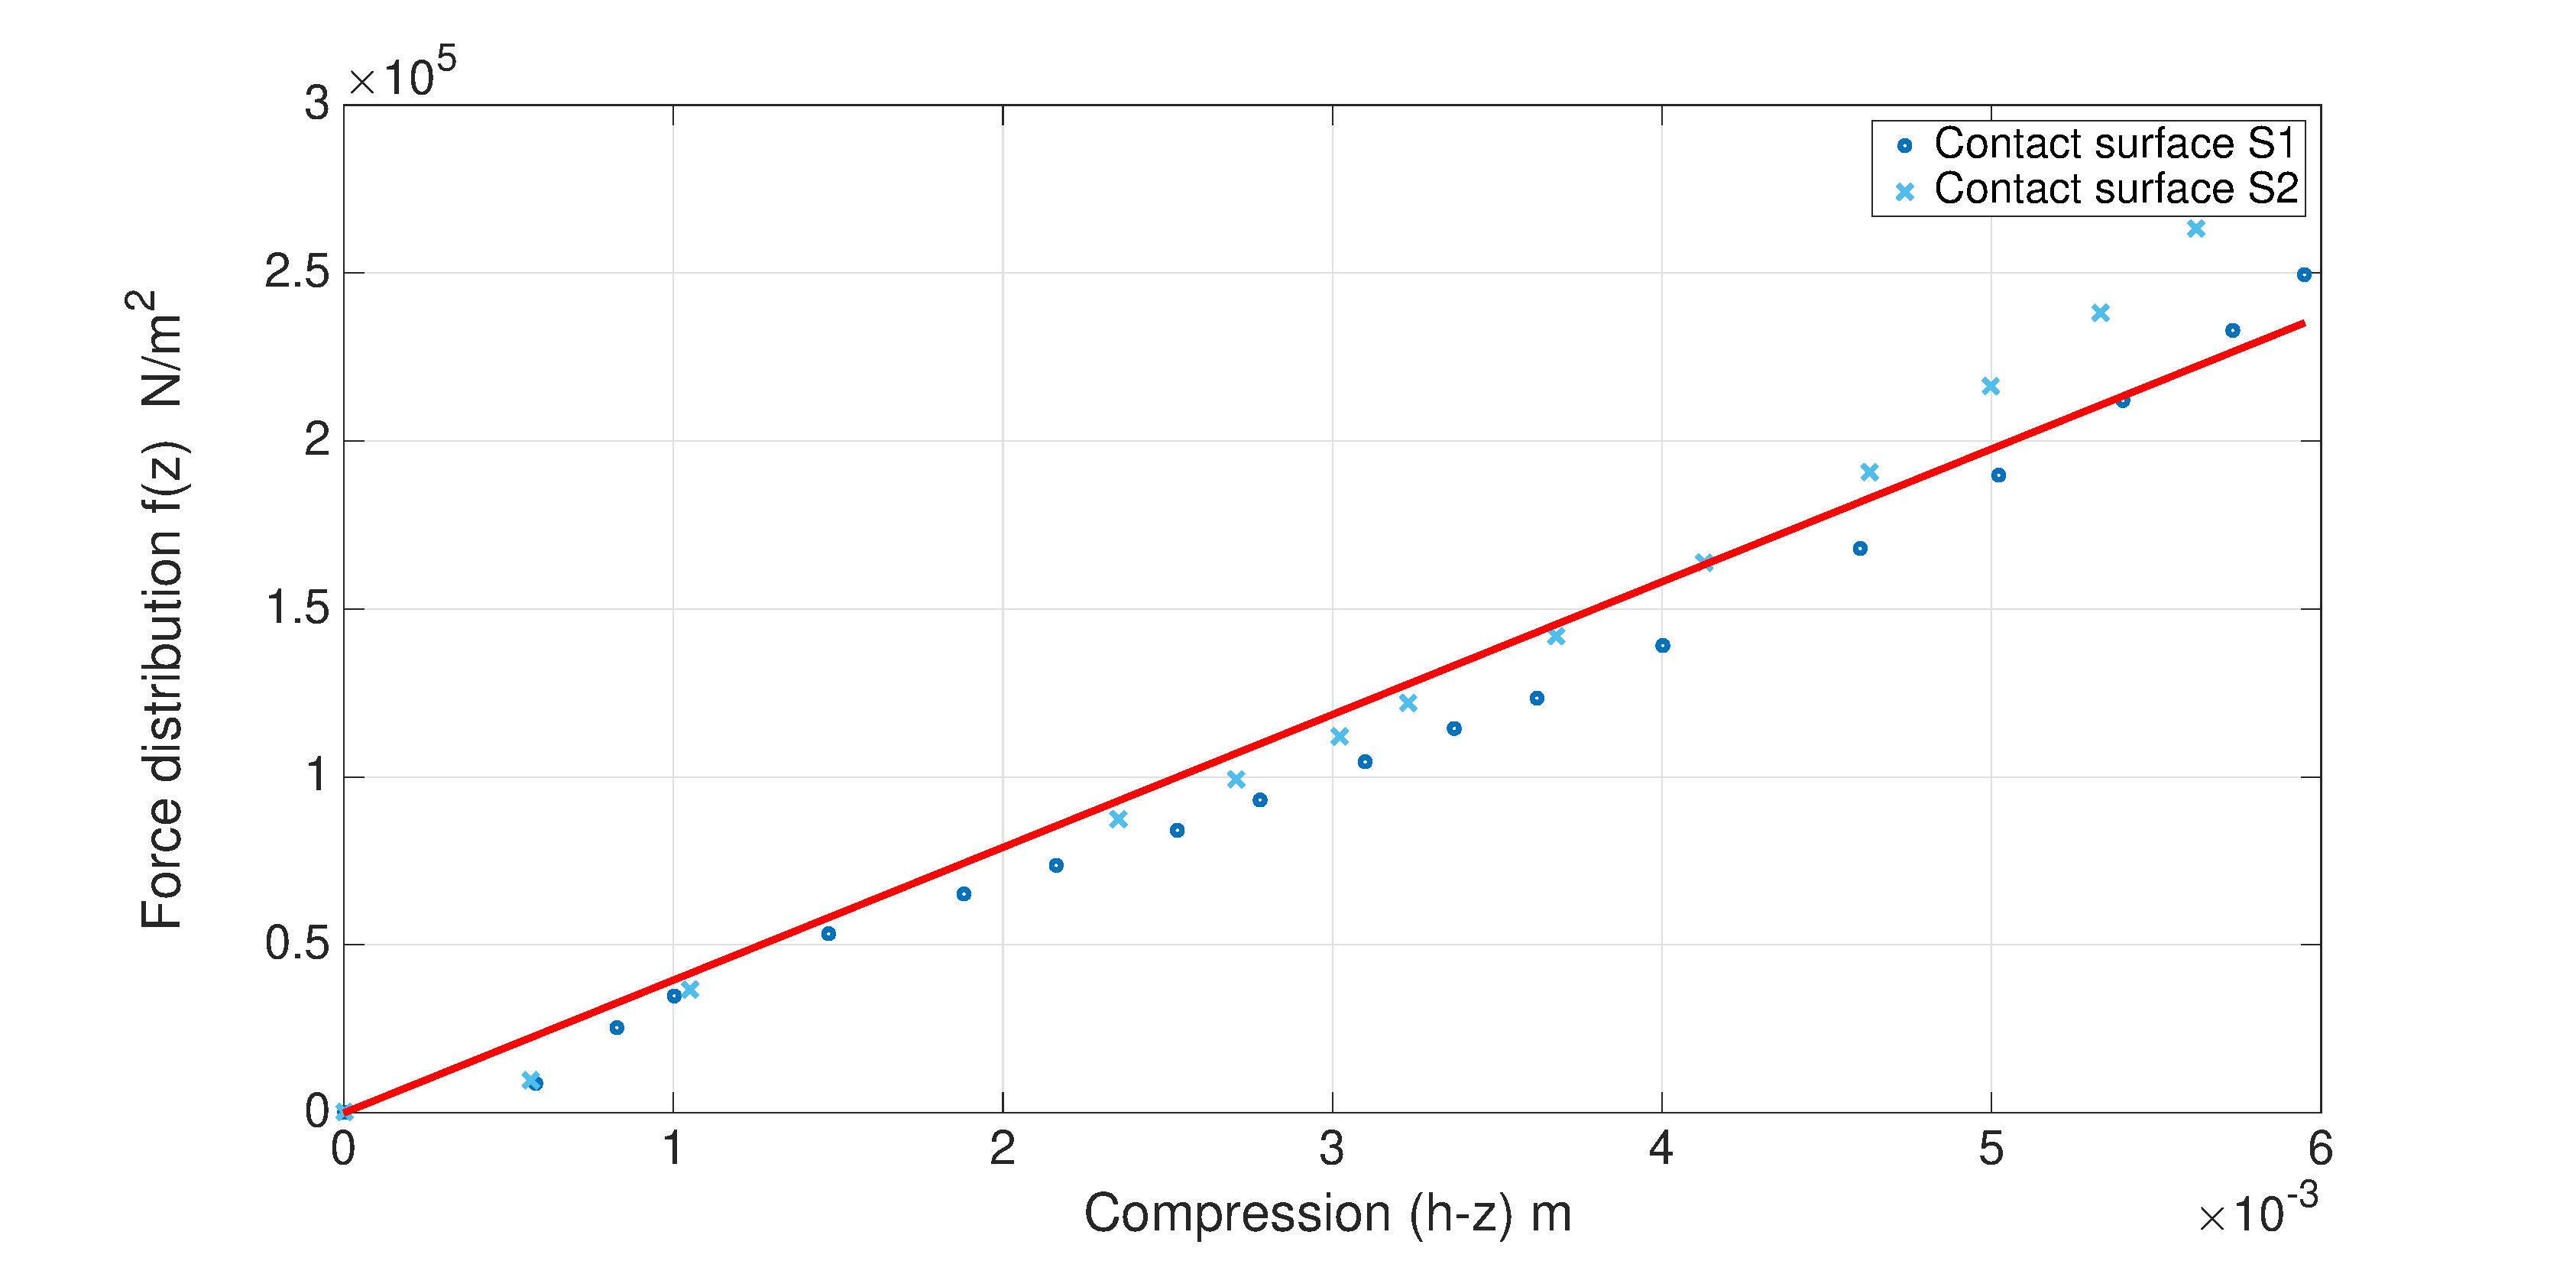
\includegraphics[width=\linewidth]{figures/estimationTests.eps}    \caption{Estimation setup}
    \label{fig:estimationResults}
    \end{center}
\end{figure}
Figure~\ref{fig:estimationResults} depicts both the measurements taken  for the two different surfaces and the approximation result. Recall that the force distribution $f(z)$ is estimated from the measurement of the contact force via  
Eq.~\eqref{fromForceToDistr3D}, i.e. 
\begin{equation}
f(z) = \frac{|F_E(z)|}{l_id_i}, \nonumber
\end{equation}
with $i \in \{1,2\}$. Hence, Figure~\ref{fig:estimationResults} points out the following facts:
\begin{itemize}
\item Assumption~\ref{hp:uniformity}.1, namely the carpet characteristics be uniform,  is well-posed. In fact, measurements taken with a larger contact surface show that the governing behavior of the force distribution $f(z)$ does not change significantly versus the contact's surface.  
\item The assumption made in Lemma~\ref{lemma3D} on the linearity of the force distribution  versus $(h-z)$ is well-posed. 
\item Since the carpet is of $h= 1 \ cm$, it shows some nonlinear effects around $(h-z)\approx 0.6 \ cm$. This threshold, which impairs the use of the model~\eqref{distributionLinear3D} to evaluate the total force-torque acting on the plate, is far from the operational condition representing a foot size in contact with the carpet.   
\end{itemize}








\newpage
\section*{Appendix}
\subsection*{Proof of Lemma~\ref{lemma3D}}
First, note that any point $p=(x,y,z)$ of the rectangular surface can be expressed as follows
\begin{equation}
\label{changeOfVariable}
p = p_M + Rp',
\end{equation}
where $R$ is the rotation matrix given by $R = (\imath,\jmath,n)$, and $p'=(u,v,0)$ any point of the rectangular surface expressed in the frame $(p_M,R)$, which implies that $u\in \left[-\frac{l}{2},\frac{l}{2}\right]$ and
$v~\in~\left[-\frac{d}{2},\frac{d}{2}\right]$. Then, we consider~\eqref{changeOfVariable} as a variable change 
\begin{subequations}
	\label{changeOfVariables}
    \begin{alignat}{2}
x &= x(u,v) \label{xUvu}
\\
y &= y(u,v)  
\label{yUvi} 
    \end{alignat}
\end{subequations}
to facilitate the process of finding the solutions to the integrals~\eqref{forceTorque3DGeneral}. Let us  remind that given a double integral of a function $g(x,y): \mathbb{R}^2 \rightarrow \mathbb{R}$, a variable change of the form~\eqref{changeOfVariables} yields 
 \begin{equation}
 \int\int g(x,y) dx dy = \int\int g(x(u,v),y(u,v)) |\det(J)|dudv, 
\end{equation}
where $J$ is the Jacobian of the variable transformation~\eqref{changeOfVariables}, i.e.

\begin{equation}
\label{generalJacobian}
J =
\begin{pmatrix}
\partial_u x &  \partial_v x  \\
\partial_u y & \partial_v y
\end{pmatrix}
\end{equation}
It is straightforward to verify that the variable change~\eqref{changeOfVariable} yields

\begin{equation}
\label{particularJacobian}
|\det(J)| = |\imath_1 \jmath_2 - \imath_2 \jmath_1| = |n^\top e_3|
\end{equation}
Once the variable change~\eqref{changeOfVariables} has been applied, the domains on which the integrals~\eqref{forceTorque3DGeneral} must be evaluated are normal with domains $u\in \left[-\frac{l}{2},\frac{l}{2}\right]$ and
$v~\in~\left[-\frac{d}{2},\frac{d}{2}\right]$. Hence, from Eqs.~ \eqref{forceTorque3DGeneral}~\eqref{distributionLinear3D}~\eqref{changeOfVariable} and~\eqref{particularJacobian}, one has
\begin{subequations}
\label{forceTorque3DGeneralVC}
    \begin{alignat}{2}
\label{eq:forcesDist3DEVC}
F &= e_3 k |n^\top e_3| \int_{-\frac{d}{2}}^{\frac{d}{2}} dv \int_{-\frac{l}{2}}^{\frac{l}{2}} (h-z_M -\imath_3 u - \jmath_3 v)  du, \\
\label{eq:torqueDist3DEVC}
M &= k |n^\top e_3|
% \int \int S(p-p_0) e_3 f(z) dx dy =
\int_{-\frac{d}{2}}^{\frac{d}{2}} dv \int_{-\frac{l}{2}}^{\frac{l}{2}}
%\begin{pmatrix}
%    y_M +\imath_2 u + \jmath_2 v - \bar{y} \\
%    x_M +\imath_1 u + \jmath_1 v - x \\
%    0
%\end{pmatrix}
(h{-}z_M {-}\imath_3 u {-} \jmath_3 v) S(p_M - \bar{p} + u \imath + v \jmath)e_3
  du.
    \end{alignat}
\end{subequations}
By computing the above integrals, one gets~\eqref{forceTorqueOn3DBentPlate}.
% \bibliographystyle{plain}
% \bibliography{references}


\end{document}
